\documentclass{beamer}

\RequirePackage{tikz}
\usetikzlibrary{shapes.misc}
\usetikzlibrary{positioning,intersections}
\usetikzlibrary{petri}
\usetikzlibrary{calc,intersections,through,backgrounds}
\usetikzlibrary{calc,decorations.pathmorphing,patterns}

\usetheme{PUT}
\title{Not-So-Linked Solution to the\\Linked Data Mining Challenge 2016}
\author{Jedrzej Potoniec}
\date{30.05.2016}
\institute{Institute of Computing Science, Poznan University of Technology}
\begin{document}
\begin{frame}
\titlepage
\end{frame}
\begin{frame}{Agenda}
\begin{enumerate}
\item Feature construction
\item Machine learning workflow
\item Insight into ML model
\end{enumerate}
\end{frame}
%TODO irregularities?


%In the beginning, we planned to extract features from \emph{DBpedia} using \emph{Fr-ONT-Qu} \cite{frontqu} from \emph{RMonto} \cite{rmonto}, a plugin to \emph{RapidMiner} \cite{rapidminer}.
%Unfortunately, the most promising feature discovered this way was a binary information if an album has a review score from \emph{Pitchfork}\footnote{\url{http://pitchfork.com/}} or not.
%After investigating, we discovered that during the extraction from \emph{Wikipedia} to \emph{DBpedia} a relation between a reviewing website and a review score has been lost.
%Consider triples for the \emph{Strange Mercy} album\footnote{\url{http://dbpedia.org/page/Strange_Mercy}}: there are 11 triples with a property \texttt{dbp:rev} and a few triples with properties like \texttt{dbp:rev10score}, but one has absolutely no way to connect scores to the reviewing websites.
%The very same problem happens with properties \texttt{dbp:title} (12 values) and \texttt{dbp:length} (11 values): it is impossible to decide on a length for a concrete track.
%
%We thought about using \emph{Yago} \cite{yago}, but it seemed to lack review information.
%We also tried to use \emph{DBTune}\footnote{\url{http://dbtune.org/}}, as suggested by the challenge website, but it rendered out to be a dead end.
%For example, \emph{MusicBrainz data}, the most interesting dataset there, is a \emph{Service Temporarily Unavailable} for a very long time now.
\begin{frame}{Linked datasets: DBTune}
\begin{tikzpicture}
\node {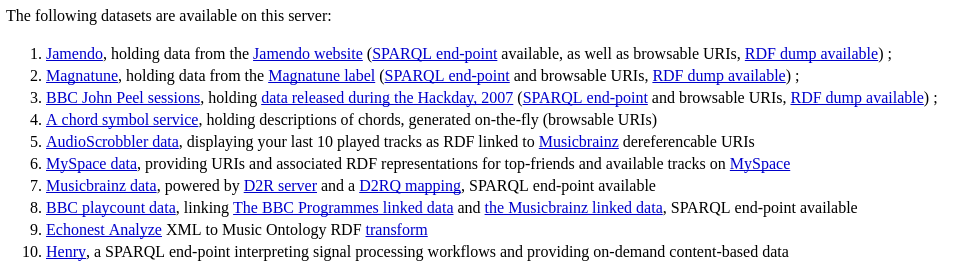
\includegraphics[scale=.6]{dbtune.png}};
\draw[thick,red,->] (-7.8,-.85) -- +(.5,0);
\end{tikzpicture}
\only<2->
{

\includegraphics[width=\textwidth]{musicbrainz.png}
}
\end{frame}

\begin{frame}{Linked datasets: DBpedia}
\url{https://en.wikipedia.org/wiki/Strange_Mercy?oldid=667760297}

\includegraphics[width=.32\textwidth]{strange_mercy1.png}
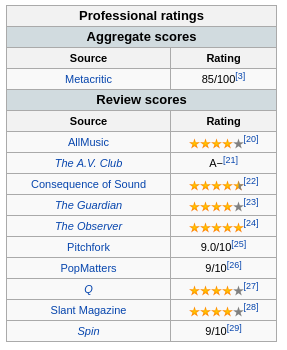
\includegraphics[width=.32\textwidth]{strange_mercy2.png}
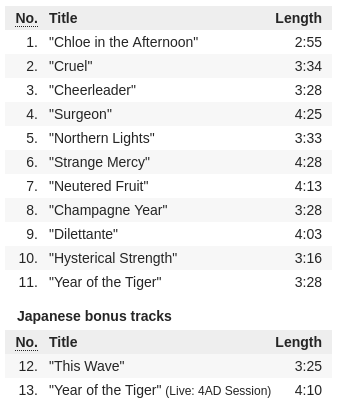
\includegraphics[width=.32\textwidth]{strange_mercy3.png}
\end{frame}

\begin{frame}{Linked datasets: DBpedia}
\url{http://dbpedia.org/resource/Strange_Mercy}

\includegraphics[width=.32\textwidth]{strange_mercy1.png}
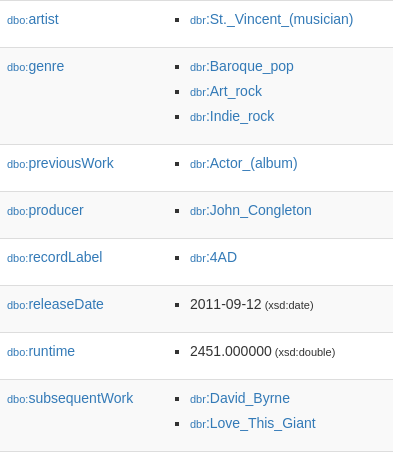
\includegraphics[width=.5\textwidth]{dbpedia1.png}
\end{frame}

\begin{frame}{Linked datasets: DBpedia}
\url{http://dbpedia.org/resource/Strange_Mercy}
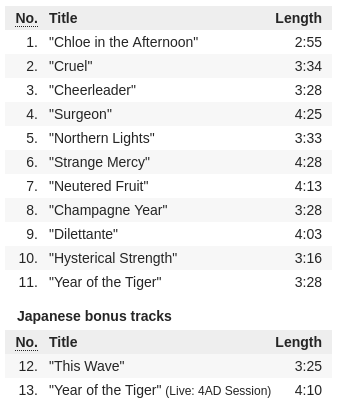
\includegraphics[width=.32\textwidth]{strange_mercy3.png}
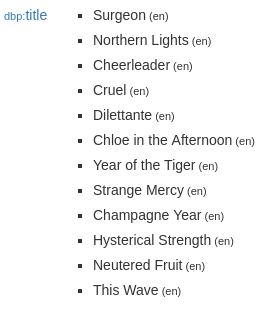
\includegraphics[width=.32\textwidth]{dbpedia3a.png}
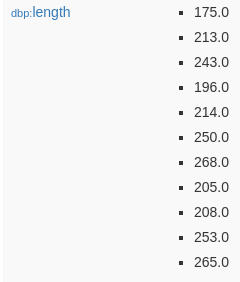
\includegraphics[width=.32\textwidth]{dbpedia3b.png}
\end{frame}

\begin{frame}{Linked datasets: DBpedia}
\url{http://dbpedia.org/resource/Strange_Mercy}
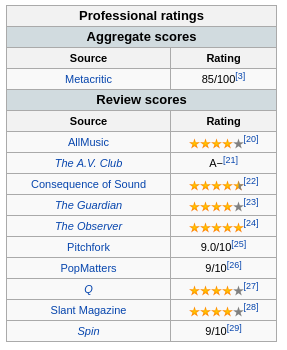
\includegraphics[width=.32\textwidth]{strange_mercy2.png}
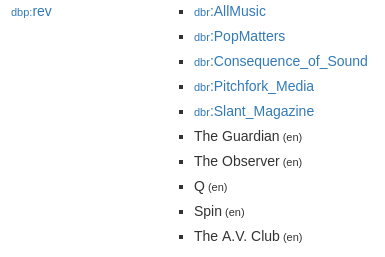
\includegraphics[width=.32\textwidth]{dbpedia2a.png}
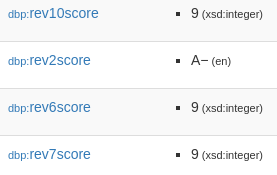
\includegraphics[width=.32\textwidth]{dbpedia2b.png}
\end{frame}

\end{document}